\documentclass[10pt,a4paper,twocolumn]{article}
\usepackage[brazil]{babel}
\usepackage[utf8]{inputenc}
\usepackage[T1]{fontenc}
\usepackage[margin=2cm,columnsep=0.65cm]{geometry}
\usepackage{graphicx,amsmath,microtype,url}
\usepackage[numbers,sort&compress]{natbib}
\usepackage[font=footnotesize,labelfont=bf]{caption}
\usepackage{titlesec}
\titleformat{\section}{\normalfont\bfseries\normalsize}{\thesection.}{.4em}{}
\titlespacing*{\section}{0pt}{1.1ex plus .2ex}{.5ex}
\setlength{\parindent}{1em}
\setlength{\parskip}{0pt}
\setlength{\textfloatsep}{8pt}
\setlength{\dbltextfloatsep}{8pt}
\setlength{\floatsep}{6pt}
\setlength{\bibsep}{1pt}
\title{\vspace{-1.4em}\large\bfseries Escala e desigualdades no acesso estimado a pronto-atendimentos nas capitais brasileiras}
\author{\normalsize Lia Sucupira\\[-1pt]\small Universidade de Fortaleza}
\date{}
\begin{document}
\maketitle
\vspace{-1.2em}

\section{Problema}
Contagens municipais podem esconder diferenças de acesso entre bairros. Investigamos como a oferta de pronto-atendimentos varia com população e renda e como se distribuem as distâncias estimadas pelas ruas nas capitais brasileiras. No cadastro CNES, consideramos estabelecimentos ativos do tipo 73 que atendem o SUS, incluindo UPAs, PAs, AMA 24h e SPAs.

Leis de escala relacionam indicadores urbanos à população \citep{bettencourt2021}. Para serviços públicos, um modelo de otimização prevê densidade de unidades proporcional à densidade populacional elevada a $2/3$ \citep{gastner2006}. Essa previsão depende de hipóteses e é usada aqui como referência, não como prova de que os serviços reais estejam bem ou mal localizados. Estudos intraurbanos também destacam a relação entre distribuição de serviços, população e rede viária \citep{xu2020}.

\section{Dados e métodos}
Integramos o cadastro CNES/OpenDataSUS (24/10/2026), população, setores e renda média do responsável pelo domicílio do Censo 2022 (IBGE), e ruas do OpenStreetMap/Geofabrik. A renda não é per capita. Há 245 unidades SUS e 274 unidades do tipo 73 nas capitais; Aracaju, sem unidade desse tipo no recorte, não entra nos ajustes. As regressões usam as outras 26 capitais. Corrigimos coordenadas e reunimos polígonos repetidos: cada setor tem população e área oficial contadas uma vez.

Representamos cruzamentos por nós e trechos dirigidos por arestas. Para cada setor, o Dijkstra encontra o menor custo total até uma unidade: ligação do ponto do setor à rua + percurso pela rede + ligação da unidade à rua. Assim, a unidade escolhida minimiza a soma inteira, não apenas o trecho entre nós. Distância é estimada para carro e não equivale a tempo de viagem. Excluímos setores sem moradores, sem rota finita ou com ligação do ponto à rua acima de 2 km; restam 90\,985 setores e 45\,770\,048 moradores. Em Todos, o PA Ilha de Maré está no cadastro, mas seus dois setores (1.178 moradores) não passam pelo filtro de 2 km; sem área válida, não entram nos ajustes de densidade.

Ajustamos por mínimos quadrados em logaritmos: (L1) número de unidades por capital em função da população; (L2) densidade de unidades $D_j=m_j/A_j$ em função da densidade de moradores $\rho_j=P_j/A_j$ na área de atendimento $j$; e um modelo conjunto que inclui renda média $\bar r_j$, com coeficiente $\delta$. Áreas são definidas pelos setores atribuídos à unidade mais acessível; unidades ligadas ao mesmo nó compartilham uma área e são contadas separadamente em $m_j$. Há 245 áreas e unidades em SUS; em Todos, 272 áreas representam 273 unidades (uma das 274 não tem setor válido associado). O modelo de renda reúne capitais, sem efeitos fixos. Intervalos percentis de 95\% usam 2.000 reamostragens bootstrap de capitais (L1) ou áreas (L2 e renda), semente 42 \citep{melo2014}.

Por fim, calculamos curvas complementares de distância e Gini ponderados pela população. Para comparar capitais, dividimos distância pela média da própria cidade. Quartis de renda e densidade são definidos dentro de cada capital. A L3 é descritiva, sem estimar expoente de cauda \citep{newman2005}.

\begin{figure*}[t]
\centering
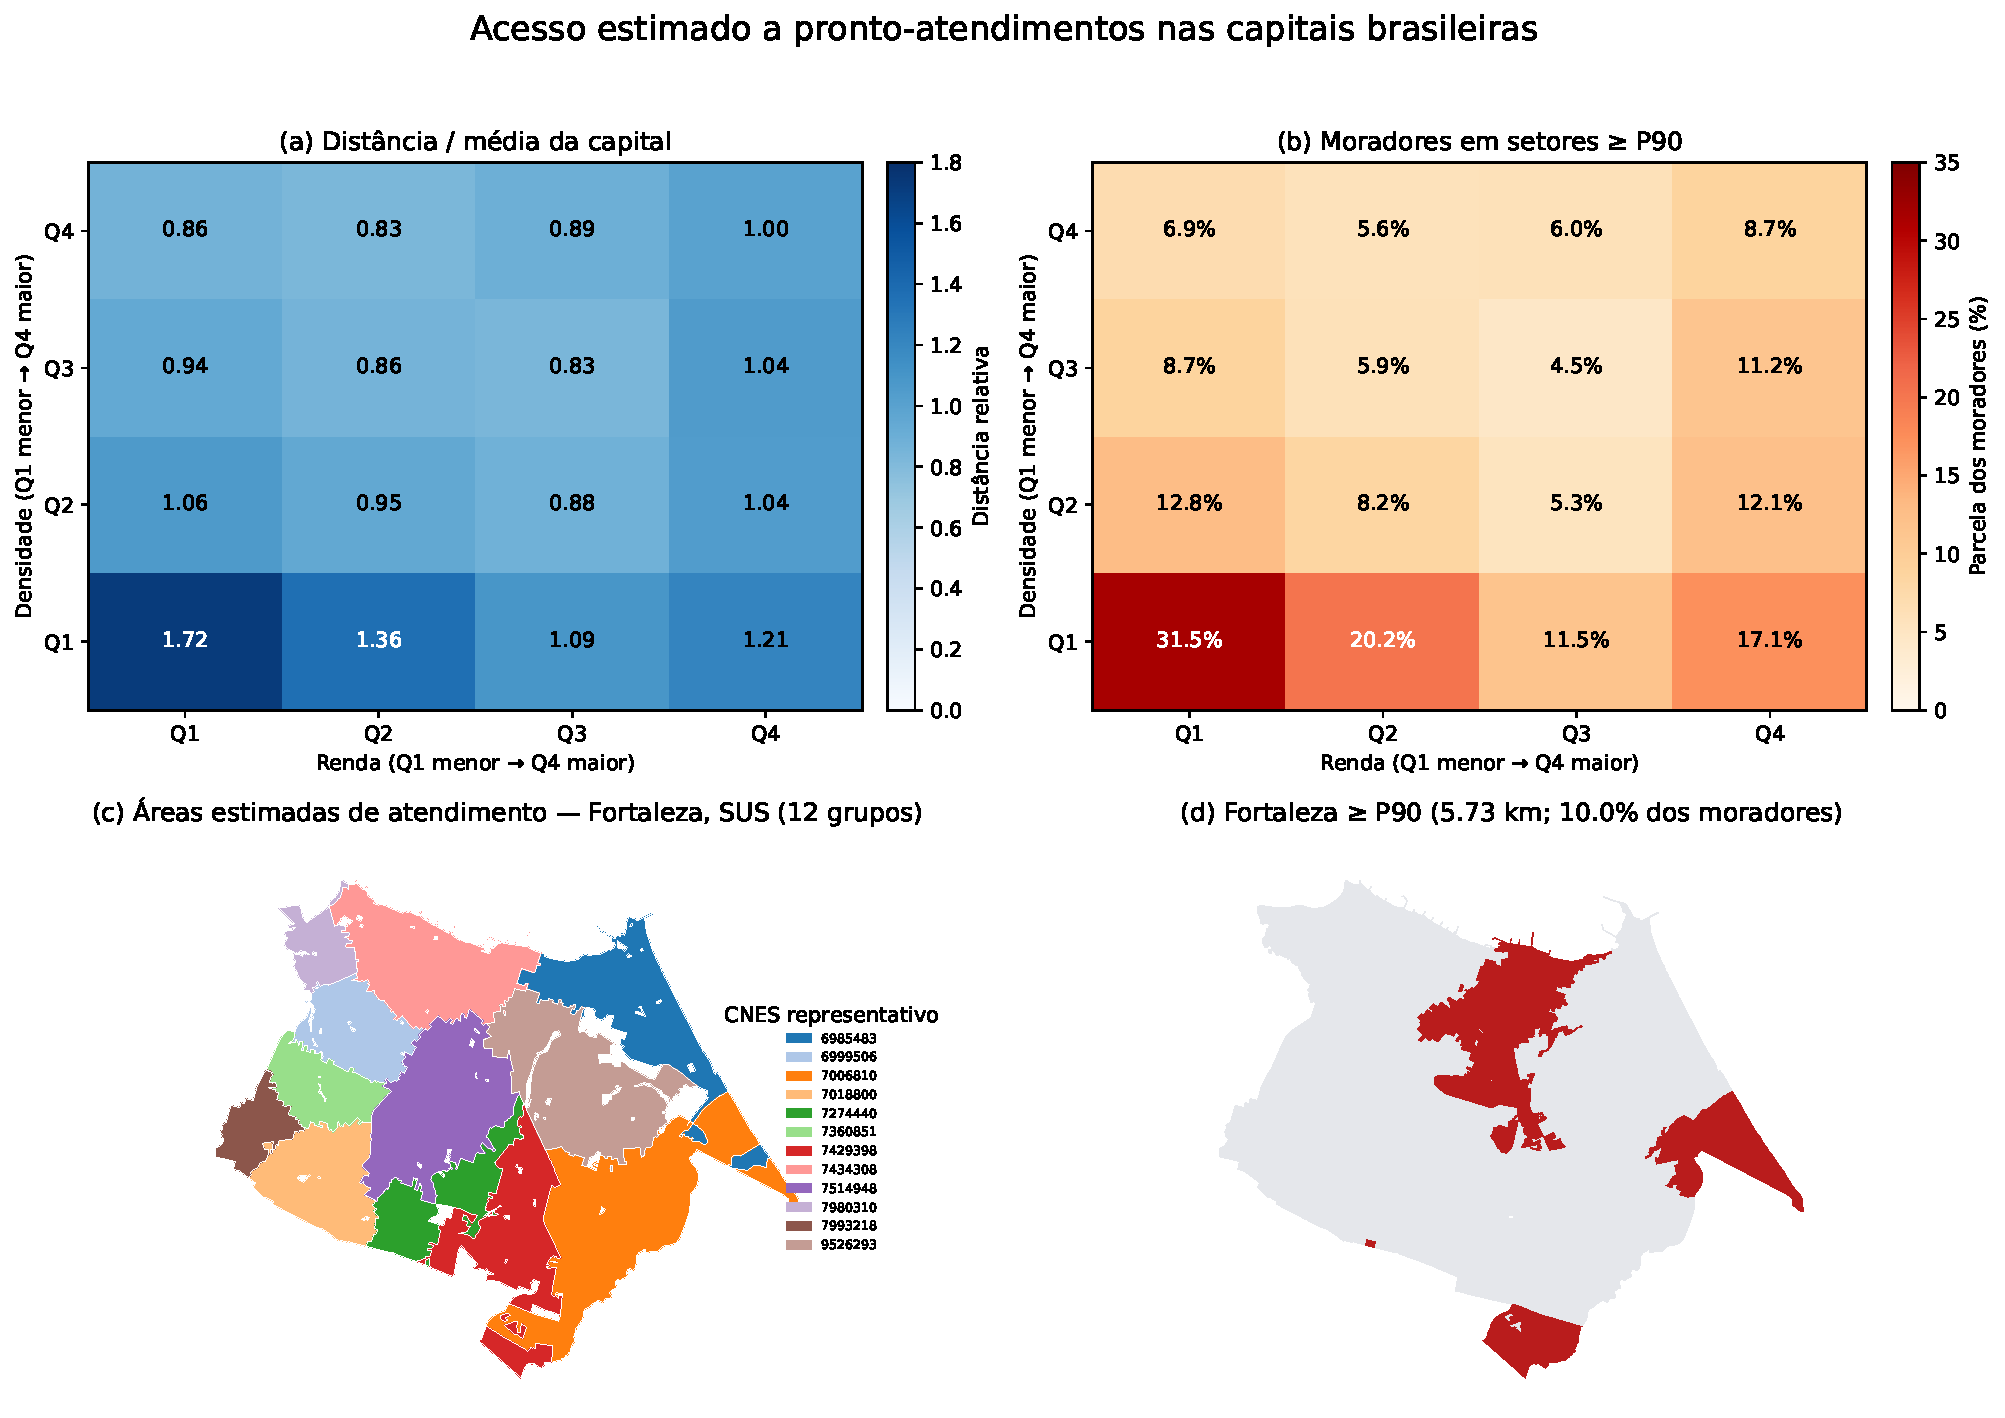
\includegraphics[width=0.97\textwidth]{../figuras/final/figura_principal.pdf}
\caption{Acesso estimado ao pronto-atendimento SUS. (a) Distância relativa média nos 16 grupos de renda e densidade, agregados entre capitais; 1 equivale à média da cidade. (b) Moradores em setores com distância igual ou acima do P90 de cada capital; o corte é relativo à própria cidade. (c) Áreas estimadas de atendimento em Fortaleza (12 grupos). (d) Setores de Fortaleza com distância igual ou acima do P90 SUS, 5,73 km. Quartis são calculados por capital.}
\label{fig:principal}
\end{figure*}

\section{Resultados e conclusão}
Na L1, $\beta=0{,}870$ (IC 95\% $[0{,}693;\,1{,}021]$); o intervalo inclui 1, portanto o ajuste é compatível com proporcionalidade entre população e unidades. Com todos os estabelecimentos, $\beta=0{,}883$ ($[0{,}695;\,1{,}051]$).

Na L2, $\alpha=0{,}861$ ($[0{,}797;\,0{,}935]$) em SUS e $0{,}899$ ($[0{,}834;\,0{,}973]$) em Todos. Os intervalos ficam acima de $2/3$ e abaixo de 1: a relação observada aumenta mais com a densidade de moradores que a referência de dois terços, mas menos que proporcionalmente. Isso não demonstra, por si só, ineficiência nem localização ótima.

No modelo de renda SUS, $\delta=-0{,}196$ ($[-0{,}353;\,-0{,}029]$). Mantida a densidade populacional, renda duas vezes maior se associa a oferta prevista 0{,}87 vez a oferta de referência, cerca de 13\% menor. Em Todos, $\delta=0{,}029$ ($[-0{,}122;\,0{,}188]$), com intervalo que inclui zero; não há associação clara nesse recorte. São associações, não efeitos causais, e o modelo mistura diferenças dentro e entre capitais.

A tabela de renda e densidade revela uma situação que a média conjunta não resume: no grupo de menor renda e menor densidade, a distância relativa média é 1{,}72 e 31{,}5\% dos moradores estão em setores acima do P90 de suas capitais. Em Fortaleza, o P90 SUS é 5,73 km e 10{,}0\% da população válida está em setores nesse corte. Como os moradores são contados por setor, essa fração pode passar de 10\%. P90 é um marcador relativo para identificar as maiores distâncias de cada cidade, não um padrão clínico. As curvas e o Gini descrevem a distribuição das distâncias, sem teste formal de lei de potência.

Os resultados mostram por que contagens municipais e um único expoente não bastam para descrever o acesso: as distâncias variam entre grupos sociais e cidades. O expoente L2 reúne áreas de 26 capitais e não descreve necessariamente a relação dentro de cada cidade; além disso, $D_j$ e $\rho_j$ compartilham a área no denominador, o que pode gerar associação matemática. Os intervalos reamostram áreas, sem modelar explicitamente o agrupamento por capital nem a dependência espacial, e devem ser lidos como incerteza exploratória. As estimativas também dependem dos pontos representativos dos setores, das ligações à rua, da cobertura da rede OSM, dos limites municipais e do corte de 2 km. Estabelecimentos são contados sem informação de capacidade, demanda, qualidade ou tempo real de viagem; 1.178 moradores dos setores associados ao PA Ilha de Maré ficam fora das análises de distância por esse filtro. A renda é agregada e não mede diretamente necessidade clínica. Portanto, identificamos padrões e diferenças de acesso estimado, mas não provamos que uma unidade esteja em localização ruim nem que a renda cause as diferenças.

{\footnotesize
\bibliographystyle{unsrtnat}
\bibliography{referencias}
}
\end{document}
